\pdfcompresslevel=0
\documentclass[a4paper]{article}

\usepackage{pgfplots}
\usepgfplotslibrary{patchplots}

\begin{document}

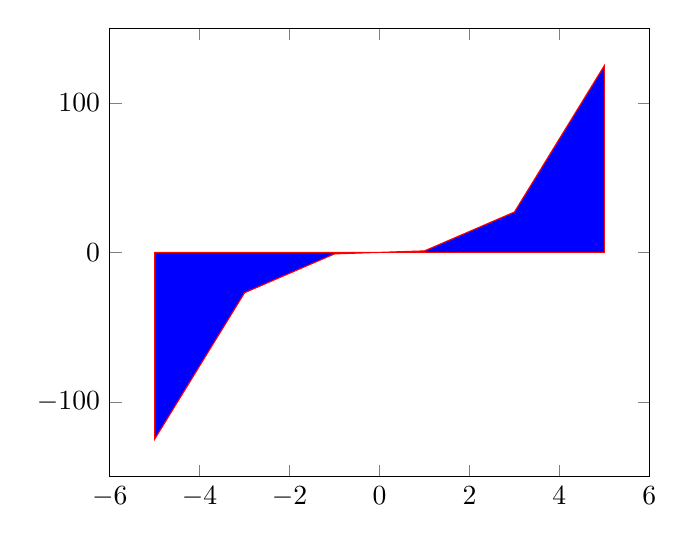
\begin{tikzpicture}
%\tracingcommands=2\tracingmacros=2
	\begin{axis}
	\addplot[mesh,red,fill=blue,samples=6,point meta=none] {x^3} \closedcycle;	
	\end{axis}
\end{tikzpicture}

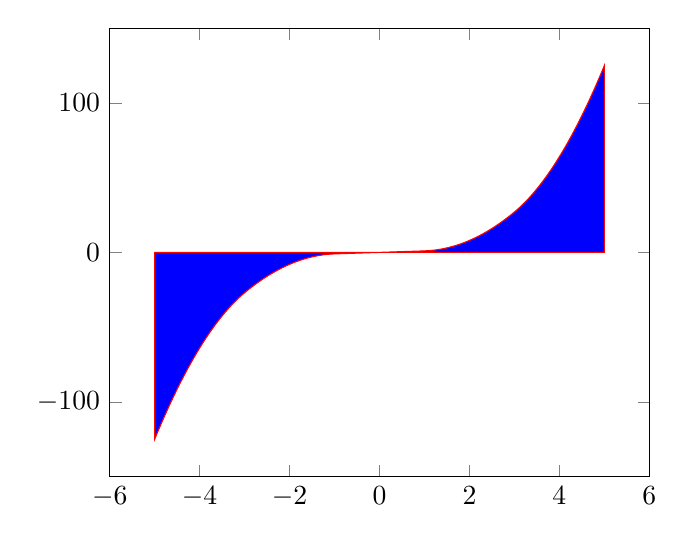
\begin{tikzpicture}
%\tracingcommands=2\tracingmacros=2
	\begin{axis}
	\addplot[mesh,red,patch type=quadratic spline,patch type sampling,fill=blue,samples=6,point meta=none] {x^3} \closedcycle;	
	\end{axis}
\end{tikzpicture}

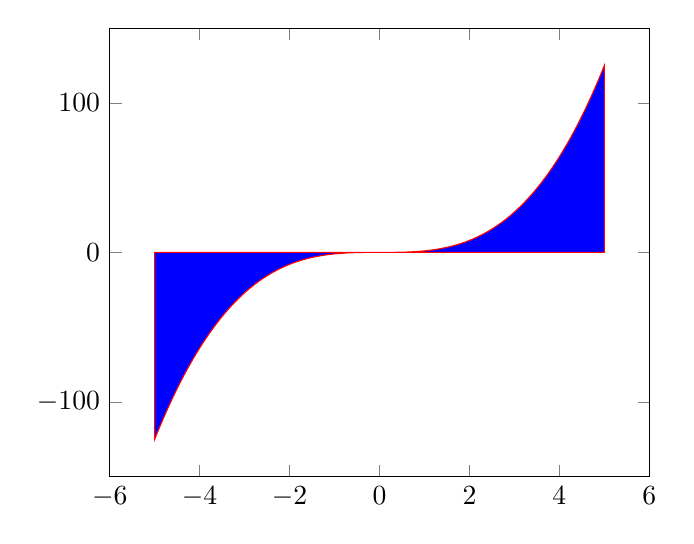
\begin{tikzpicture}
%\tracingcommands=2\tracingmacros=2
	\begin{axis}
	\addplot[mesh,red,patch type=cubic spline,patch type sampling,fill=blue,samples=6,point meta=none] {x^3} \closedcycle;	
	\end{axis}
\end{tikzpicture}

\begin{tikzpicture}
%\tracingcommands=2\tracingmacros=2
	\begin{axis}
	\addplot[mesh,samples=6] {x^3};	
	\end{axis}
\end{tikzpicture}


%--------------------------------------------------
% \begin{tikzpicture}
% \begin{axis}
% \addplot[patch,patch type=cubic spline,fill=blue]coordinates{(0,0)(3,1)(1,.5)(2,.5)} \closedcycle;
% \end{axis}
% \end{tikzpicture}
%-------------------------------------------------- 

\end{document}

